\RequirePackage{fix-tudscrfonts}

\documentclass[t,nototalpages,useheader=false]{tudbeamer}

\usepackage[beamer,
            ocontsyntax=modal,
            bibresource=../references.bib,
            biblatex=true,
            bibstyle=authoryear]{preamble20171016}


%% defining colors
\definecolor{skyblue}{rgb}{0.80, 0.80, 1.00}
\definecolor{turquoise}{rgb}{0.00, 0.80, 0.60}
\definecolor{gray}{gray}{0.59}
\definecolor{darkgray}{gray}{0.40}

\colorlet{text}{black!30!hks_41_k_100}
\colorlet{frametitle}{gray}
\colorlet{framesubtitle}{black}
\colorlet{accent}{turquoise}
\colorlet{alink}{skyblue}
\colorlet{vlink}{lightgray}
\colorlet{alert}{hks_07_k_100}
\colorlet{titlebackground}{hks_41_k_100}

\setbeamercolor{normal text}{fg=text}
\setbeamercolor{structure}{fg=text}
\setbeamercolor{alerted text}{fg=alert}
\setbeamercolor{frametitle}{fg=frametitle}
\setbeamercolor{framesubtitle}{fg=framesubtitle}


\renewcommand*{\framesubtitle}[1]{\textcolor{frametitle}{\textbf{#1}}}

\makeatletter

%% logo

\def\logo@front{TUDCDrosi/logo_weiss}
\def\logo@default{TUDCDrosi/logo_blau}
\ifx\pdfoutput\undefined%
\else%
  \ifx\pdfoutput\relax%
  \else%
    \ifcase\pdfoutput%
    \else%
      \def\logo@front{TUDCDrosi/TU_Logo_SW}%
      \def\logo@default{TUDCDrosi/TU_Logo_SW}%
    \fi%
  \fi%
\fi
\def\conceptlogo@front{TUDCDrosi/DDC-weissf}
\def\rosilogo@front{TUDCDrosi/rosi-inv}
\def\rosilogo@default{TUDCDrosi/rosi}

\renewcommand\maketitle{%
  % \beamertemplateshadingbackground{darkblue}{darkblue}
  \setbeamercolor{normal text}{bg=titlebackground}
  % Kopf-/Fusszeile fuer Titel
  \setbeamertemplate{headline}{%
    \vskip6.15mm%
    \color{white}%
    \setlength{\arrayrulewidth}{0.3pt}%
    \begin{tabular*}{\paperwidth}[b]{l@{\extracolsep\fill}}
      % TUD-Logos
      \hspace*{3.0mm}%
      \color{white}%
      \includegraphics[height=7.81mm,draft=false]{\logo@front}%
      \hspace*{6.96cm}
      \includegraphics[height=7.81mm,draft=false]{\rosilogo@front}%
      \\[1.2mm]\hline
      \hspace*{11.76mm}%
      \rule[-0.8mm]{0pt}{2.47mm}%
      \def\@@dummyComma{}%
      \rule{0pt}{5.8pt}%
      \textbf{\@einrichtung }\ifx\@einrichtung\@empty\else\def\@@dummyComma{ }\fi%
      \ifx\@fachrichtung\@empty%
      \else%
      \@@dummyComma\@fachrichtung%
      \ifx\@institut\@empty\else\def\@@dummyComma{, }\fi%
      \ifx\@professur\@empty\else\def\@@dummyComma{, }\fi%
      \fi%
      \ifx\@institut\@empty\else\@@dummyComma\@institut%
      \ifx\@professur\@empty\else\def\@@dummyComma{, }\fi%
      \fi%
      \ifx\@professur\@empty\else\@@dummyComma\fi%
      \@professur\\[-1pt]\hline
    \end{tabular*}\hspace{-\paperwidth}%
  }%
  \setbeamertemplate{footline}{%
    \parbox[t][9.63mm]{\paperwidth}{%  \parbox[t][9.63mm]{\paperwidth}{
      \vspace*{-13.63mm}%
      \rule{13.86mm}{0pt}%
      \small%
      \color{white}%
      \insertdatecity%
      \ifx\insertdatecity%
      \empty%
      \else%
      \ifx\insertdate%
      \empty%
      \else%
      , %
      \fi%
      \fi%
      \insertdate%
      \hfill%
      \parbox[b][13mm]{13mm}{
        \includegraphics[height=13mm,draft=false]{\conceptlogo@front}%
      }
    }
    % \vspace{8mm}
    % \includegraphics[height=9.63mm]{\conceptlogo@front}%
  }%
  \frame{\titlepage}%
  % Kopf-/Fusszeilen fuer restliche Folien
  \setbeamertemplates%
}

\setbeamertemplate{title page}{
  \color{white}%
  \vfill%
  \usebeamerfont*{title}%
  \vskip2ex plus1ex minus1ex%
  \MakeUppercase{\inserttitle}%
  % \inserttitle%
  \vfill%
  \ifx\insertsubtitle\empty%
  \else%
  \usebeamerfont*{subtitle}%
  \insertsubtitle%
  \vfill%
  \fi%
  \normalfont\large%
  \insertauthor%
  \vfill%
  \vfill%
}



\makeatother


\einrichtung{Institute of Theoretical Computer Science\ }
\professur{Chair for Automata Theory}

\title{Context Reasoning for Role-Based Models}
\author{Stephan Böhme}
\date{27.10.2017}
\datecity{Dresden}

\begin{document}

\makeatletter
\renewcommand{\@slide}{}
\makeatother

\begin{frame}
%  \vspace*{-2cm}
  \frametitle*{Motivation}
  \framesubtitle{What is a Role?}
  
  \begin{minipage}{0.45\linewidth}
   
    \begin{itemize}
    \item Modelling concept from OOP introduced by Bachman in 1973
    \item Classification of roles with 26 \emph{Features} including identity, behaviour,
      relationships, players, \dots{} and about Contexts and Constraints
      {\tiny(\cite{KuLG-SLE14,Stei-DKE00})}
    \end{itemize}
  \end{minipage}\hfill
  \begin{minipage}{0.5\linewidth}
    \begin{tikzpicture}[cls/.style={draw,rectangle,minimum width=2cm,minimum height=5mm}]
      \only<1-2>{\node[cls] (a) at (0,1.5) {\only<1>{Person}\only<2>{\textit{Customer}}};}
      \only<3->{\node[cls] (a) at (-1.8,1.5) {Person};}
      \only<3->{\node[cls] (b) at (1.8,1.5) {Company};}
      \node[cls] (c) at (-1.8,0) {\only<1,3->{\textit{Customer}}\only<2>{Person}};
      \node[cls] (d) at (1.8,0) {\only<1,3->{\textit{Supplier}}\only<2>{Company}};
      \only<1->{\draw (c) -- (a) -- (d);}
      \only<3->{\draw (c) -- (b) -- (d);}
    \end{tikzpicture}
  \end{minipage}

\uncover<4->{
\framesubtitle{Requirements for modern Software Systems:}

\begin{minipage}{1.0\linewidth}
  \begin{itemize}
  \item Adaptability \only<5->{\alert{\qquad $\to$ \smash{Roles} allow for dynamic changes of the
        system.}}
  \item High expressiveness \only<5->{\alert{\qquad $\to$ Roles increase separation of
        concerns.}}
  \item Longevity \only<5->{\alert{\qquad $\to$ Roles enable updating running applications.}}
  \end{itemize}
\end{minipage}

}
  
\end{frame}

\begin{frame}
  \frametitle*{\RBS}
  \vspace*{-2ex}
  \begin{itemize}
  \item Software systems that use the notion of roles
  \item Focus on: Compartment Role Object Model (CROM), {\tiny(\cite{KuLG-SLE14})}
    \begin{itemize}
    \item Well-defined semantical foundation {\tiny(\cite{KBG-SLE15})}
    \end{itemize}
  \end{itemize}
  %
  %\vfill
  \only<2-4>{
    \framesubtitle{Key properties of roles:}
    \begin{itemize}
    \item Roles depend on the context.
    \item Contexts, `players' and roles themselves have each their own identity.
    \item Roles change over time.
    \end{itemize}
  }
  %
  %\vfill
  \only<3-4>{
    \framesubtitle{Problems:}
    \begin{itemize}
    \item Large systems/models hard to comprehend
    \item Modelling errors stay undetected \only<4>{\qquad\alert{$\rightarrow$ Logic-based
          formalisms}}
    \end{itemize}
  }

  \only<5>{
    \begin{minipage}[t]{0.5\linewidth}
      \fontsize{7}{8}\selectfont
      \framesubtitle{Key properties of roles:}
      \begin{itemize}
      \item Roles depend on the context.
      \item Contexts, `players' and roles themselves have each their own identity.
      \item Roles change over time.
      \end{itemize}
    \end{minipage}%
    \begin{minipage}[t]{0.5\linewidth}
      \fontsize{7}{8}\selectfont
      \framesubtitle{Problems:}
      \begin{itemize}
      \item Large systems/models hard to comprehend
      \item Modelling errors stay undetected
      \item[\follows] Logic-based formalisms
      \end{itemize}
    \end{minipage}
    \vfill
    \framesubtitle{Requirements on logical formalism}
    \begin{itemize}
    \item Decidable reasoning tasks
    \item Model contexts and ternary relation of role-playing
    \item Ability to handle \emph{rigid}, i.e.\ context-independent, knowledge
    \item 
    \end{itemize}
    
  }
  
  %\vfill
\end{frame}

\begin{frame}
  \frametitle*{Overall Workflow -- Outline}
\end{frame}


\begin{frame}
  \frametitle*{Running Example - Banking Application}
  \vfill
  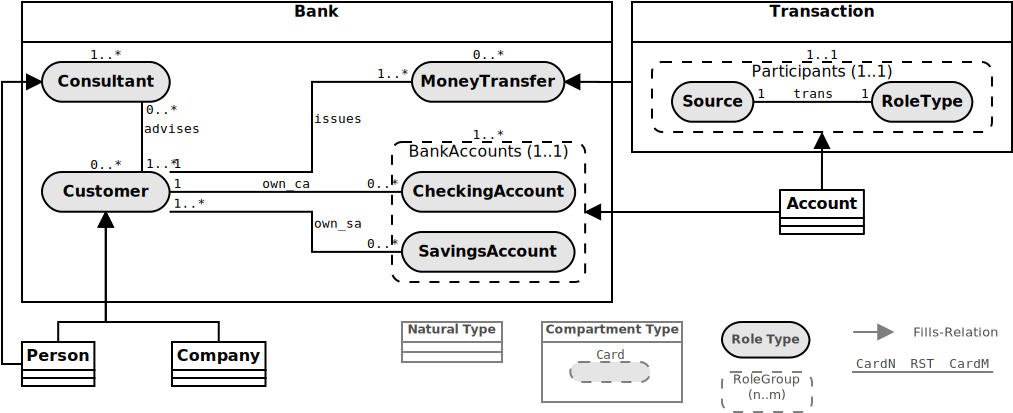
\includegraphics[width=\textwidth]{Bank-full-constraints}
  \vfill
\end{frame}























\begin{frame}[c]
  \begin{center}
    \Large Thank you for your attention!\\[2ex]
    Any questions?
  \end{center}
\end{frame}

\begin{frame}[t,allowframebreaks]
  \frametitle*{References}
  \printbibliography
\end{frame}



\end{document}


%%% Local Variables: 
%%% mode: latex
%%% TeX-master: t
%%% reftex-default-bibliography: ("../references.bib")
%%% End: 